\chapter{Vector Spans and Independence}
Think back to a time when you played with blocks. If you had two blocks, you couldn't make many shapes out of them. With three, you had a few more options. With a dozen you were able to make many more shapes. In the world of blocks, a span would be all the things you could make with a given set of blocks. 

A vector span is similar, but in a mathematical sense. If I give you the coordinates for a vector and ask you to make everything you can from that vector using only the original vector, the result is the span. You can scale the vector, add it to itself, anything that is a linear combination of only that vector. As with the blocks, you'll find what you can make from one vector is limited. The span will be a line. But when you are given two or more vectors to "play" with, you will be able to create much more. The span will be larger than in the case of having only one vector. The size of the span (sometimes referred to as a subspace) will depend on whether the vectors are linearly independent or dependent. 

\section{Overview: Independence and Dependence}
A set of linearly independent vectors means that no vector is a combination of any other vector. Let's look at these three:
$$[1 0 0]$$
$$[0 1 0]$$
$$[0 0 1]$$

If you scale each vector as much as possible, the span encompasses the entire 3D real space. 

A set of linearly dependent vectors means one or more of the vectors can be written as a combination of one of the vectors.

For example:
$$v_1 = [7 -2 2]$$
$$v_2 = [14 -4 4]$$

You can see that $v_2$ is $2*v_1$. They are linearly dependent. This is a simple example, but when you encounter very large matrices, it won't be as obvious. You will learn computational techniques for figuring out independence.

Vector spans have practical applications in a number of fields. Computer graphics and physics are two of them. For example, in space travel, knowing the vector span is essential to calculating a slingshot maneuver that will give spacecraft a gravity boost from a planet. For this, you'd need to know the gravity vector of the planet relative to the sun and the velocity vectors that characterize the spacecraft. Engineers would use this information to figure out the trajectory angle that would allow the spacecraft to achieve a particular velocity in the desired direction. The span constrains the set of successful solutions.

\section{Formal Definitions}
Now that you have a sense of what a span is, it's time for the formal mathematical definition. A vector span is the collection of vectors obtained by scaling and combining the original set of vectors in all possible proportions.  Formally, if the set $S = \{v_1, v_2, ..., v_n\}$ contains vectors from a vector space $V$, then the span of $S$ is given by:

\begin{equation}
\text{Span}(S) = \{a_1v_1 + a_2v_2 + ... + a_nv_n : a_1, a_2, ..., a_n \in \mathbb{R}\}
\end{equation}

This means that any vector in the Span$(S)$ can be written as a linear combination of the vectors in $S$.

\section{Independent Vectors}
A set of vectors $S = \{v_1 v_2 ... v_n\}$ is  linearly independent if the only solution to the equation:
$$a_1v_1 + a_2v_2 + ... + a_nv_n = 0$$
is 
$$a_1 = a_2 = ... = a_n = 0$$ 

This means that no vector in the set can be written as a linear combination of the other vectors.

If there exists a nontrivial solution (i.e., a solution where some $a_i \neq 0$), then the vectors are said to be linearly dependent. This means that at least one vector in the set can be written as a linear combination of the other vectors.

The concept of vector independence is fundamental to the study of vector spaces, bases, and rank. You'll learn more about these concepts in future modules. 

\subsection{Dependent Vectors}
Let's start by looking at two vectors. 

$$v_1 = \begin{bmatrix}
			2 \\
			4
		\end{bmatrix}$$
$$v_2 = \begin{bmatrix}
			-14 \\
			-28
\end{bmatrix}$$

These two vectors are dependent because $v_2 = -7*v_2$. This is an obvious example but let's show it mathematically. If linearly independent, the two vectors must satisfy:

	$$v_1a_1 + v_1a_2 = 0$$
	$$v_2a_1 + v_2a_2 = 0$$

which is:
	$$2a_1 -14a_2 = 0$$
	$$4a_1 -28a_2 = 0$$

To solve, multiply the top equation by -2 and add it to the bottom: 
$$2a_1 - 14a_2 = 0 $$
$$ 0  + 0     = 0 $$

The bottom equation drops out. Now  solve for $a_1$ in the remaining equation:
$$a_1 = -7a_2$$
As you can see, one vector is a multiple of another. $$a_1 \neq a_2 \neq 0$$

\subsection{Independent Vectors}
Let's see if these two vectors are independent.
$$v_1 = \begin{bmatrix}
1 \\
0
\end{bmatrix}$$
$$v_2 = \begin{bmatrix}
0 \\
-1
\end{bmatrix}$$

To be independent,the two vectors must satisfy:
	$$v_1a_1 + v_1a_2 = 0$$
	$$v_2a_1 + v_2a_2 = 0$$
	
which is:
$$\begin{bmatrix}
	a_1 + 0*a_2 \\
	0*a_1 + a_2
\end{bmatrix}$$

So:
$$a_1 = a_2 = 0$$
These vectors are not only independent, but they are orthogonal (perpendicular) to one another. You'll learn more about orthogonality later.

Here is an example whose solution isn't as obvious. You can solve using Gaussian elmination.
$$v_1 = [2 1]$$
$$v_2 = [1 -6]$$

Rewrite as a system of equations:
$$a_1*2 + a_2*1 = 0 $$
$$a_1*1 + a_2*(-6) = 0$$

First swap the equations to that the the top equation has a coefficient of 1 for $a_1$:
$$a_1 - 6a_2 = 0$$ 
$$2a_1 + a_2 = 0$$ 
Next multiply row 1 by -2 and add it to row 2:
$$a_1 - 6a_2 = 0$$ 
$$0  - 11a_2 = 0$$ 

Multiply row 2 by 1 divided by 11.
$$a_1 - 6a_2 = 0$$ 
$$0 + a_2 = 0$$ 

Back substitute $a_2$ solution into the first equation:
$$a_1  = 0$$
$$a_2 = 0$$ 
Therefore $a_1 = a_2 = 0$ and the two vectors are linearly independent.

\begin{Exercise}[title={Vector Independence}, label=vector_independence]
    Are these vectors independent? 
$$\begin{matrix}[2 & 1  & 4]\end{matrix}$$
$$\begin{matrix}[2  & -1  & 2]\end{matrix}$$ 
$$\begin{matrix}[0  & 1  & -2]\end{matrix}$$
Show your work.
\end{Exercise}

\begin{Answer}[ref=vector_independence]
    Rewrite as a system of equations:
        $$\begin{matrix}
			2*a_1 +2*a_2 + 0*a_3 = 0 \\
			1*a_1 - 1*a_2 + 1*a_3 = 0 \\
			4*a_1 + 2*a_2 - 2*a_3 = 0
		  \end{matrix} $$
	Simplify
		$$\begin{matrix}
			2a_1 +2*a_2 = 0 \\
			a_1 - a_2 + a_3 = 0 \\
			4a_1 + 2a_2 - 2a_3 = 0
		  \end{matrix} $$
	Swap row 2 and 1:
		$$\begin{matrix}
			a_1 - a_2 + a_3 = 0 \\
			2a_1 + 2*a_2 = 0 \\
			4a_1 + 2a_2 - 2a_3 = 0
		  \end{matrix} $$
	Multiply row 1 by -2 and add to row 2:
	   $$\begin{matrix}
			a_1 - a_2 + a_3 = 0 \\
			0 +  3*a_2 - 2a_3  = 0 \\
			4a_1 + 2a_2 - 2a_3 = 0
		  \end{matrix} $$
	Multiply row 1 by -4 and add to row 3:	
	    $$\begin{matrix}
			a_1 - a_2 + a_3 = 0 \\
			0 + 3*a_2 -2a_3 = 0 \\
			0 + 6a_2 - 6a_3 = 0
		  \end{matrix} $$
	Multiply row 2 by -4 and add to row 3:
	   $$\begin{matrix}
			a_1 - a_2 + a_3 = 0 \\
			0 + 3*a_2 -2a_3 = 0 \\
			0 + 0 - 2a_3 = 0
		  \end{matrix} $$
	Multiply row 3 by -1 and add to row 2:
		$$\begin{matrix}
			a_1 - a_2 + a_3 = 0 \\
			0 + 3*a_2 + 0 = 0 \\
			0 + 0 - 2a_3 = 0
		\end{matrix} $$
    Divide row 3 by -2 and row 2 by $\frac{1}{3}$:
    	$$\begin{matrix}
			a_1 - a_2 + a_3 = 0 \\
			0 +  a_2 +0  = 0 \\
			0  + 0  + a_3 = 0
		\end{matrix} $$
	Backsubstitute $a_2$ and $a_3$ into row 1:
	 	$$\begin{matrix}
			a_1 + 0 + 0 = 0 \\
			0 +  a_2 + 0   = 0 \\
			0   + 0  + a_3 = 0
		\end{matrix} $$
	 Therefore $$a_1 = a_2 = a_3 = 0$$.
\end{Answer}
    
\section{Checking for Linear Independence Using Python}  
One way to use python to check for linear independence is to use the linalg.solve() function to solve the system of equations. You need to create an array that contains the coefficients of the variable and a vector that contains the values on the right-side of each equation. So far, you've either been given equations that equal 0 or you've manipulated each equation to be equal to 0. 

Let's first see how to use python to solve the equations in the previous exercise. If the equations are linearly independent, then $a_1 = a_2 = a_3 = 0$

Create a file called span\_independence.Python and enter this code:
\begin{Verbatim}
import numpy as np

A = np.array([[2, 2, 0], 
              [1, -1, 1],
              [4, 2, -2]])
b = np.array([0, 0, 0])
c = np.linalg.solve(A,b)
print(c)
\end{Verbatim}
You should get this result, which shows the equations are linearly independent.
\begin{Verbatim}
[0., -0.,  0.]
\end{Verbatim}
But what happens if the equations are not independent? Let's make the first two equations dependent by making equation 1 two times equation 2. Enter this code into your file:
\begin{Verbatim}
import numpy as np

D = np.array([[2, -2, 2], 
              [1, -1, 1],
              [4, 2, -2]])
e = np.array([0, 0, 0])
f = np.linalg.solve(D,f)
print(f)

You should get many lines indicating an error. Among the spew, you should see:

raise LinAlgError("Singular matrix")
\end{Verbatim}
So while the linalg.solve() function is quite useful for solving a system of independent linear equations, raising an error is not the most elegant way to figure out if the equations are dependent. That's where the concept of a determinant comes in. You'll learn about that in the next section. But for now, let's use the  linalg.solve() function to find a solution for a set of equations known to be linearly independent.
$$4x_1 + 3x_2 - 5x_3 = 2$$
$$-2x_1- 4x_2 - 5x_3 = 5$$
$$       8x_2 + 8x_3  = -3$$
You will create a matrix that contains all the coeffients and a vector that contains the values on the right-side of the equations. 

Enter this code into your file. 
\begin{Verbatim}
G = np.array([[4, 3, -5], 
              [-2, -4, 5], 
              [8, 8, 0]])
h = np.array([2, 5, -3])

j = np.linalg.solve(G, h)
print(j)
\end{Verbatim}
You should get this answer:
\begin{Verbatim}
[2.20833333, -2.58333333, -0.18333333]
\end{Verbatim}

\section{Determinants}
The determinant of a matrix is a scalar value that indicates whether the columns of a matrix are linearly independent. For a 2D matrix, the determinant is the area of the parallelogram defined by the column vectors. For a 3D matrix, the determinant is the volume of the parallelepiped. (A six-dimensional figure formed by six paralleograms. A cube is an example.) 

Let's plot the parallelogram for this matrix:
$$
\begin{bmatrix}
2 & 0  \\
0 & 2 
\end{bmatrix}
$$

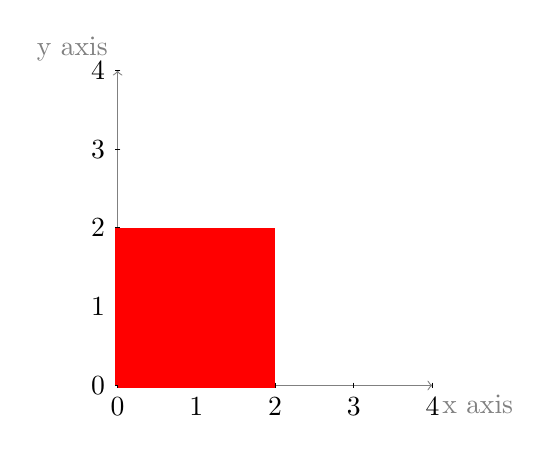
\begin{tikzpicture}
\draw[gray,->] (0,0)-- (4.0,0) node[anchor=north west] {x axis};
\draw[gray,->] (0,0)-- (0, 4.0) node[anchor=south east] {y axis};

\foreach \x in {0,1,2,3,4}
    \draw(\x cm, 1pt) -- (\x cm, -1pt) node[anchor=north] {$\x$};
\foreach \y in {0,1,2,3,4}
    \draw(1 pt,\y cm) -- (-1pt, \y cm) node[anchor=east] {$\y$};  

\draw[red, ultra thick] (0,0) -- (2,0);
\draw[red, ultra thick] (0,0) -- (0,2);
\fill[red] (0,0) rectangle(2,2);
\end{tikzpicture}
 
The formal definition for calculating the determinant of a 2 by 2 matrix is:
$$det(A) = (a*d)-(b*c)$$
where
$$A = 
\begin{bmatrix}
a & b  \\
c & d 
\end{bmatrix}
$$

For the matrix plotted above, the determinant is $(2*2)+(0*0)$. You can also see that 4.0 is the area, base (2) times height (2).

You can use the determinant to see what happens to a shape when it goes through a linear transformation. Let's scale the 2 by 2 matrix by 4:
$$
\begin{bmatrix}
8 & 0  \\
0 & 8 
\end{bmatrix}
$$
Plot it:

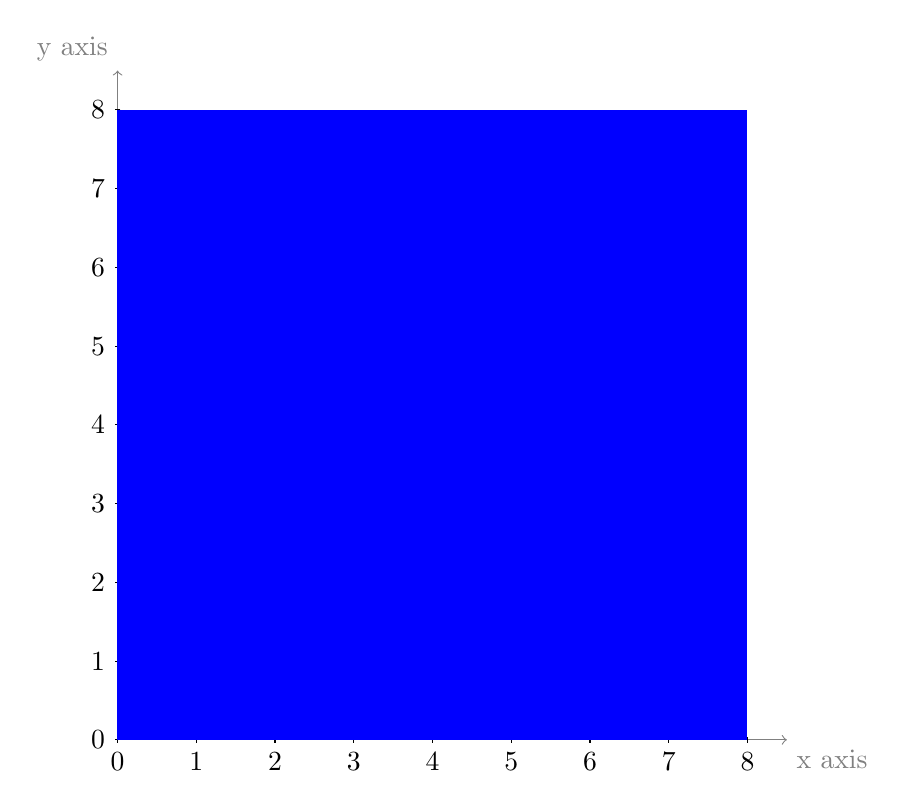
\begin{tikzpicture}
\draw[gray,->] (0,0)-- (8.5,0) node[anchor=north west] {x axis};
\draw[gray,->] (0,0)-- (0, 8.5) node[anchor=south east] {y axis};

\foreach \x in {0,1,2,3,4,5,6,7,8}
    \draw(\x cm, 1pt) -- (\x cm, -1pt) node[anchor=north] {$\x$};
\foreach \y in {0,1,2,3,4,5,6,7,8}
    \draw(1 pt,\y cm) -- (-1pt, \y cm) node[anchor=east] {$\y$};  

\draw[blue] (0,0) -- (8,0);
\draw[blue] (0,0) -- (0,8);
\fill[blue] (0,0) rectangle(8,8);


\end{tikzpicture}

Find the determinant. 

$$(8*8)+(0*0) = 64$$

You can see that scaling the matrix cubed the area.

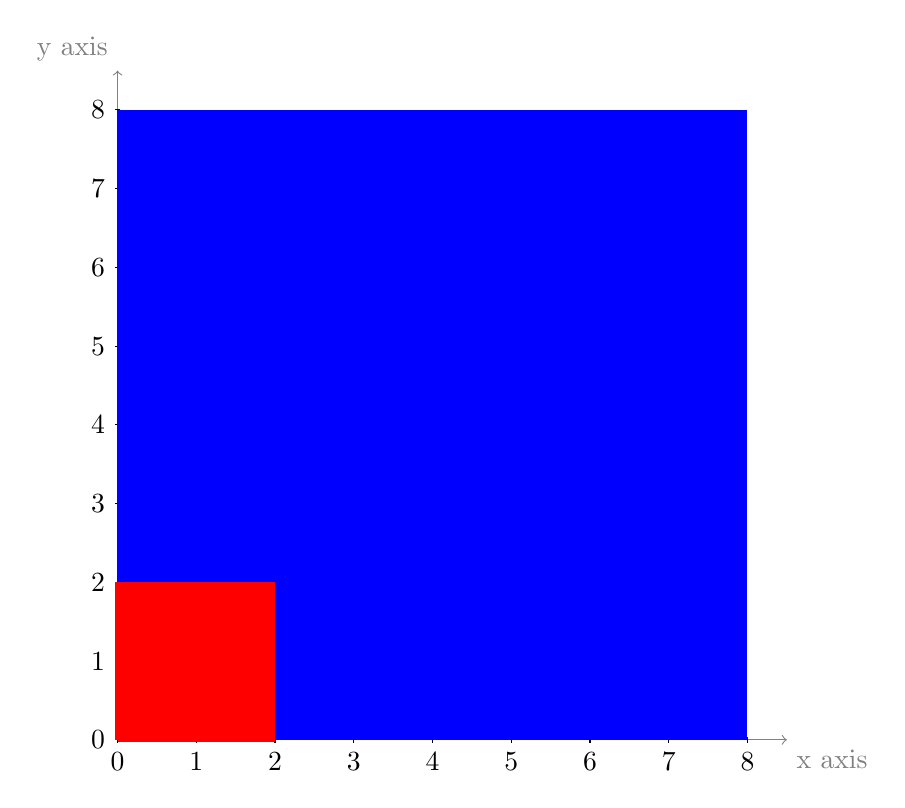
\begin{tikzpicture}
\draw[gray,->] (0,0)-- (8.5,0) node[anchor=north west] {x axis};
\draw[gray,->] (0,0)-- (0, 8.5) node[anchor=south east] {y axis};

\foreach \x in {0,1,2,3,4,5,6,7,8}
    \draw(\x cm, 1pt) -- (\x cm, -1pt) node[anchor=north] {$\x$};
\foreach \y in {0,1,2,3,4,5,6,7,8}
    \draw(1 pt,\y cm) -- (-1pt, \y cm) node[anchor=east] {$\y$};  

\draw[blue] (0,0) -- (8,0);
\draw[blue] (0,0) -- (0,8);
\fill[blue] (0,0) rectangle(8,8);

\draw[red, ultra thick] (0,0) -- (2,0);
\draw[red, ultra thick] (0,0) -- (0,2);
\fill[red] (0,0) rectangle(2,2);

\end{tikzpicture}
 
Let's plot this matrix
$$
\begin{bmatrix}
2 & 1  \\
4 & 2 
\end{bmatrix}
$$

\begin{tikzpicture}
\draw[gray,->] (0,0)-- (4.5,0) node[anchor=north west] {x axis};
\draw[gray,->] (0,0)-- (0, 4.5) node[anchor=south east] {y axis};

\foreach \x in {0,1,2,3,4}
    \draw(\x cm, 1pt) -- (\x cm, -1pt) node[anchor=north] {$\x$};
\foreach \y in {0,1,2,3,4}
    \draw(1 pt,\y cm) -- (-1pt, \y cm) node[anchor=east] {$\y$};  

\draw[red, ultra thick] (0,0) -- (4,2);
\draw[blue, ultra thick] (0,0) -- (2,1);

\end{tikzpicture}

One line overwrites the other. As you can see, the area is 0. The columns are linearly dependent.

Calculating the determinant for a 2 by 2 matrix is easy. For a larger matrix, finding the determinant is more complex and requires breaking down the matrix into smaller matrices until you reach the 2x2 form. The process is called expansion by minors. For our purposes, we simply want to first check to see if a matrix contains linearly independent rows and columns before using our Python code to solve. 

Modify your code so that is uses the $np.linalg.det()$ function. If the determinant is not zero, then you can call the $np.linalg.solve()$ function. Your code should look like this:
\begin{Verbatim}
if (np.linalg.det(D) != 0):
    j = np.linalg.solve(D,e)
    print(j)
else:
     print("Rows and columns are not independent.")
\end{Verbatim}

\section{Where to Learn More}
Watch this video on \emph {Linear Combinations and Vector Spans from Khan Academy}: \url{http://rb.gy/g1snk}

The Wolfram Demonstrations website has a fun, interactive demo where you can enter values for 2D and 3D matrices and see how the area or volume changes. 
\url{https://demonstrations.wolfram.com/DeterminantsSeenGeometrically/#more}

If you are curious about the \emph {Expansion of Minors}, see:
\url {https://mathworld.wolfram.com/DeterminantExpansionbyMinors.html}